%%%%%%%%%%%%%%%%%%%%%%%%%%%%%%%%%%%%%%%%%%%%%%%%%%%%%%%%%%%%%%%%%%%%%%%%%%%%%%%%
\section[Certification Strategy]{strategy}

%%%%%%%%%%%%%%%%%%%%%%%%%%%%%%%%%%%%%%%%%%%%%%%%%%%%%%%%%%%%%%%%%%%%%%%%%%%%%%%%
\subsection[What's in for Users]{Users}


%%%%%%%%%%%%%%%%%%%%%%%%%%%%%%%%%%%%%%%%%%%%%%%%%%%%%%%%%%%%%%%%%%%%%%%%%%%%%%%%
\begin{frame}
  \frametitle{How the Site Manager looks on HPC Education}
  \centering
  {\bcattention \bf \large Exaggeration Warning \bcattention}
  \begin{columns}
   \begin{column}{0.6\textwidth}
    \centering
    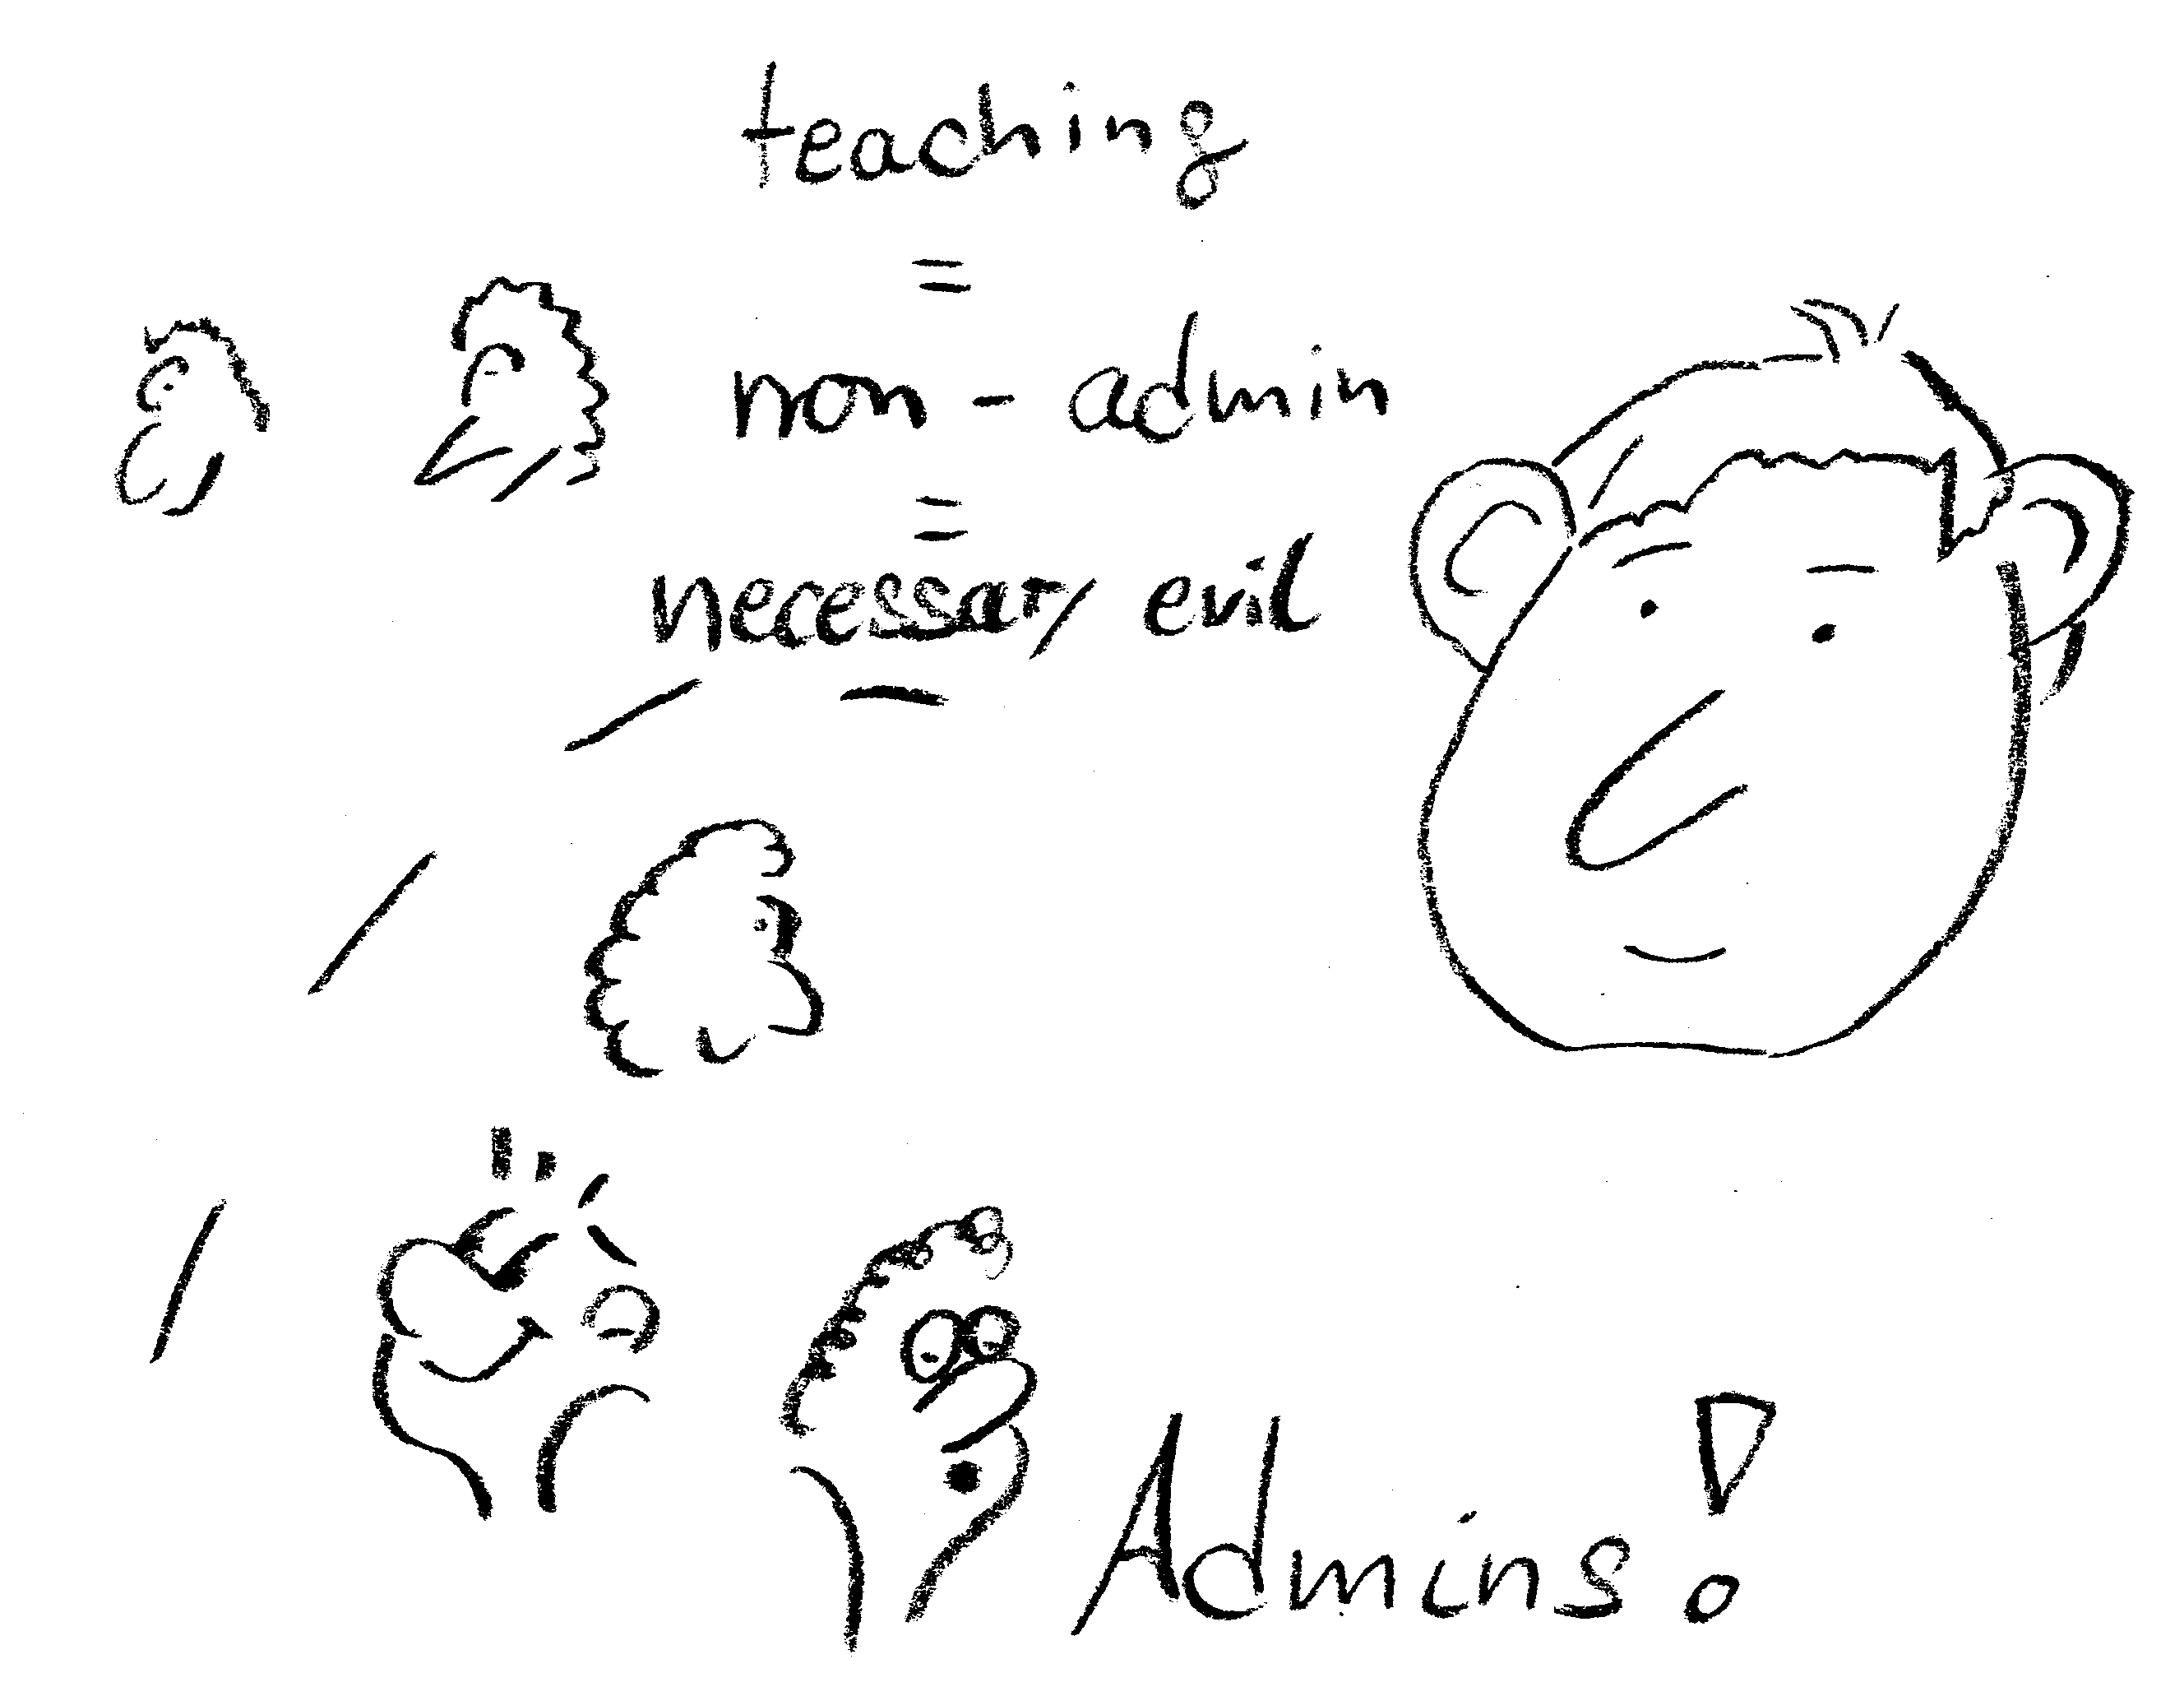
\includegraphics[width=0.8\textwidth]{images/runner}
   \end{column}
   \begin{column}{0.4\textwidth}
    \pause
    \begin{itemize}[<+->]
     \item ressources are always limited
     \item teaching ressources even more
     \item integration into HPCCF might offer more (still needed) courses
    \end{itemize}
   \end{column}
  \end{columns}
\end{frame}

%%%%%%%%%%%%%%%%%%%%%%%%%%%%%%%%%%%%%%%%%%%%%%%%%%%%%%%%%%%%%%%%%%%%%%%%%%%%%%%%
\begin{frame}
  \frametitle{HPCCF Adoption by Sites}
  \begin{columns}
   \begin{column}{0.5\textwidth}
    \centering
    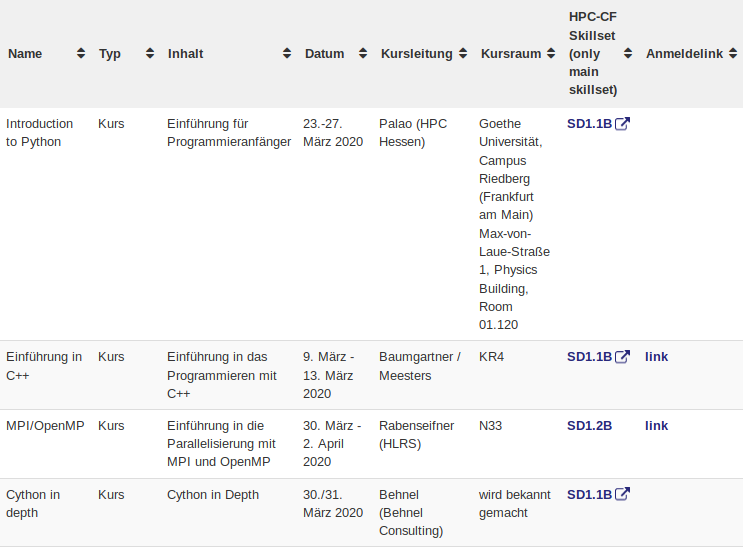
\includegraphics[width=0.8\textwidth]{images/linking_skills}\\
    \lhref{https://hpc.uni-mainz.de/kurse-und-workshops/\#bersicht}{Mainz course overview}
   \end{column}
   \begin{column}{0.5\textwidth}
     Assigning HPCCF skill labels to courses is no of cost, yet they are an asset for participating sites:
     \begin{itemize}
      \item enhanced transparency of own course portfolio
      \item own portfolio can be complemented by linking to courses nearby $\curvearrowright$ (for smaller sites) not so thin anymore
      \item with transparency a plus for users
      \item with HPCCF certificates new users may have some HPC experience other than ``submitted a job'' once
     \end{itemize}
   \end{column}
  \end{columns}
\end{frame}


%%%%%%%%%%%%%%%%%%%%%%%%%%%%%%%%%%%%%%%%%%%%%%%%%%%%%%%%%%%%%%%%%%%%%%%%%%%%%%%%
\begin{frame}
  \frametitle{How Joe User looks on HPC}
  \centering
  {\bcattention \bf \large Exaggeration Warning \bcattention}
  \begin{columns}
    \begin{column}{.5\textwidth}
     \centering
     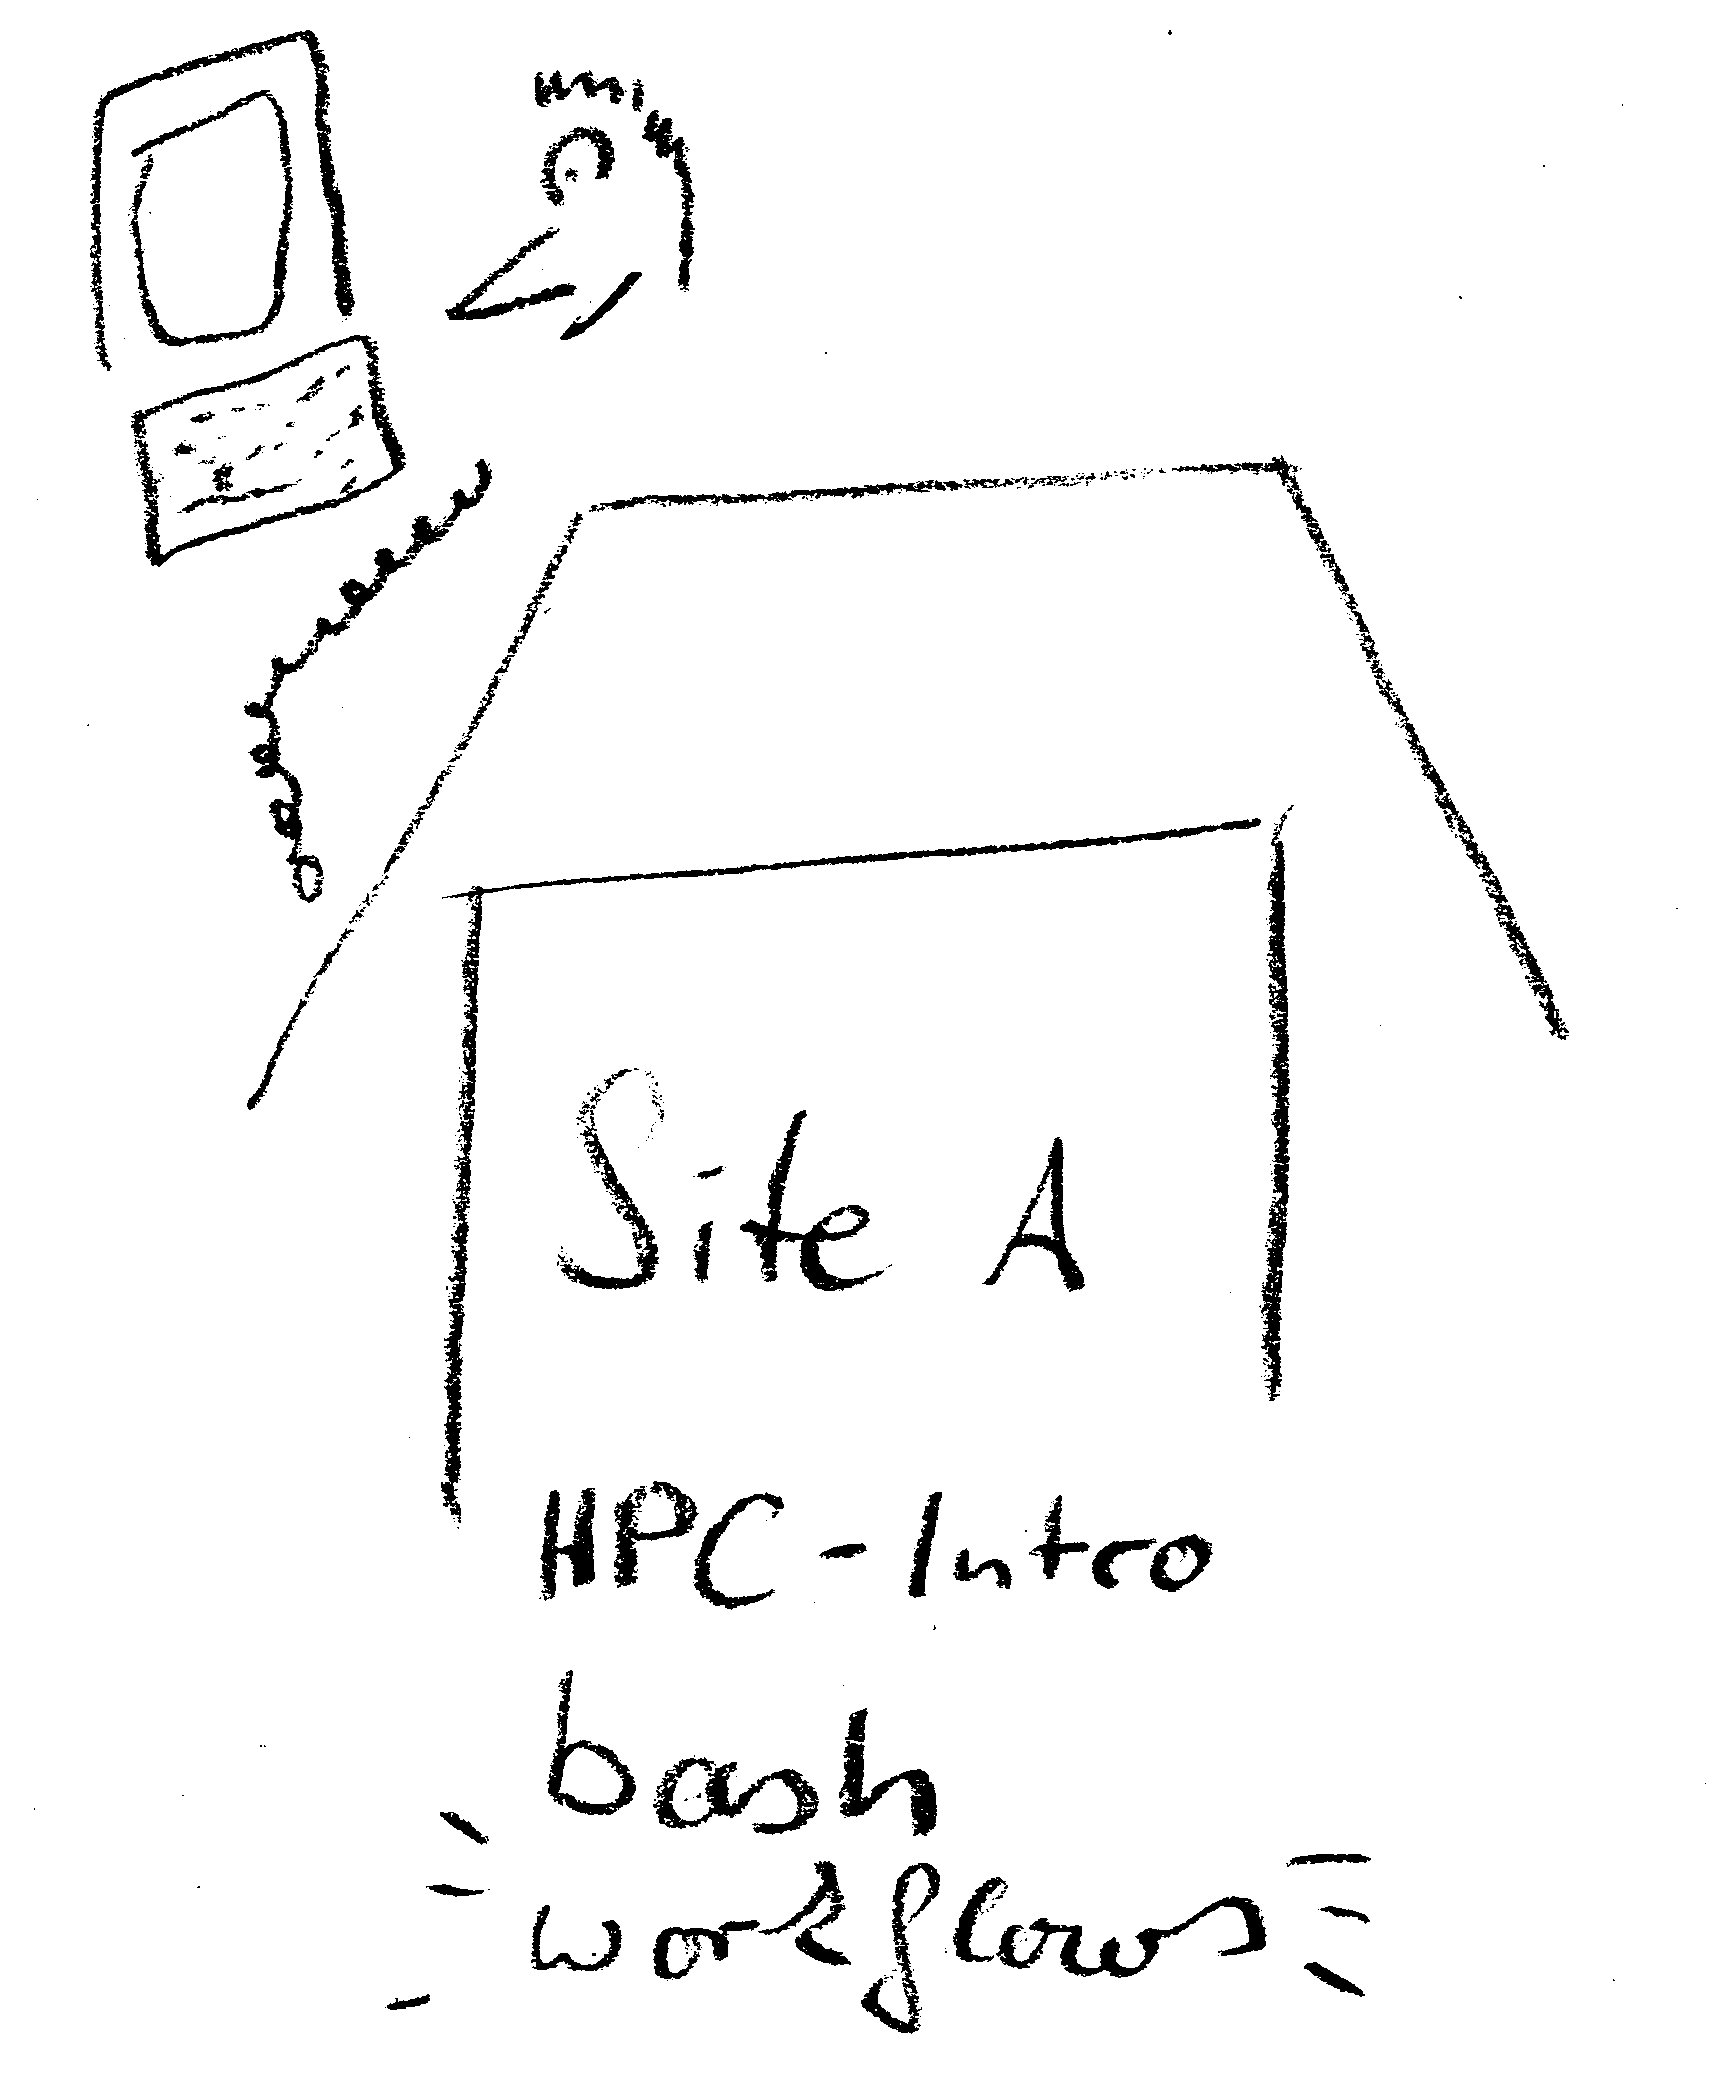
\includegraphics[width=0.7\textwidth]{images/joe}
    \end{column}
    \begin{column}{.5\textwidth}
      \pause
      Most users
      \begin{itemize}[<+->]
        \item \ldots use $3^{rd}$ party applications \ldots
        \item \ldots will need (yet not always visit) an intro course \ldots
        \item \ldots perhaps a scripting course \ldots
        \item \ldots only \emph{really} interested in workflows taylored for their need.
      \end{itemize}
      \pause
      And will never leave their site for other HPC courses!
    \end{column}
  \end{columns}
\end{frame}

%%%%%%%%%%%%%%%%%%%%%%%%%%%%%%%%%%%%%%%%%%%%%%%%%%%%%%%%%%%%%%%%%%%%%%%%%%%%%%%%
\begin{frame}
  \frametitle{HPCCF Adaption as a Plus for Newbies}
  \begin{columns}
   \begin{column}{0.5\textwidth}
    \centering
    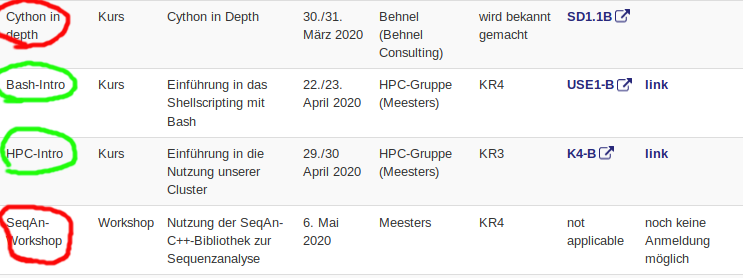
\includegraphics[width=0.8\textwidth]{images/linking_skills_users}\\
    \lhref{https://hpc.uni-mainz.de/kurse-und-workshops/\#bersicht}{Mainz course overview}
   \end{column}
   \begin{column}{0.5\textwidth}
     Assigning HPCCF skill labels to courses is no of cost, yet it will be a plus for ``only-users'':
     \begin{itemize}
      \item will broaden horizons
      \item ``\emph{Maybe} some other course might be interesting, too?''
      \item ``Hm, perhaps more knowledge in this field will be an asset when applying?''
     \end{itemize}
   \end{column}
  \end{columns}
\end{frame}


%%%%%%%%%%%%%%%%%%%%%%%%%%%%%%%%%%%%%%%%%%%%%%%%%%%%%%%%%%%%%%%%%%%%%%%%%%%%%%%%
\begin{frame}
  \frametitle{How Bruce Coder looks on HPC}
  \centering
  {\bcattention \bf \large Exaggeration Warning \bcattention}
  \begin{columns}
    \begin{column}{.6\textwidth}
      \centering
      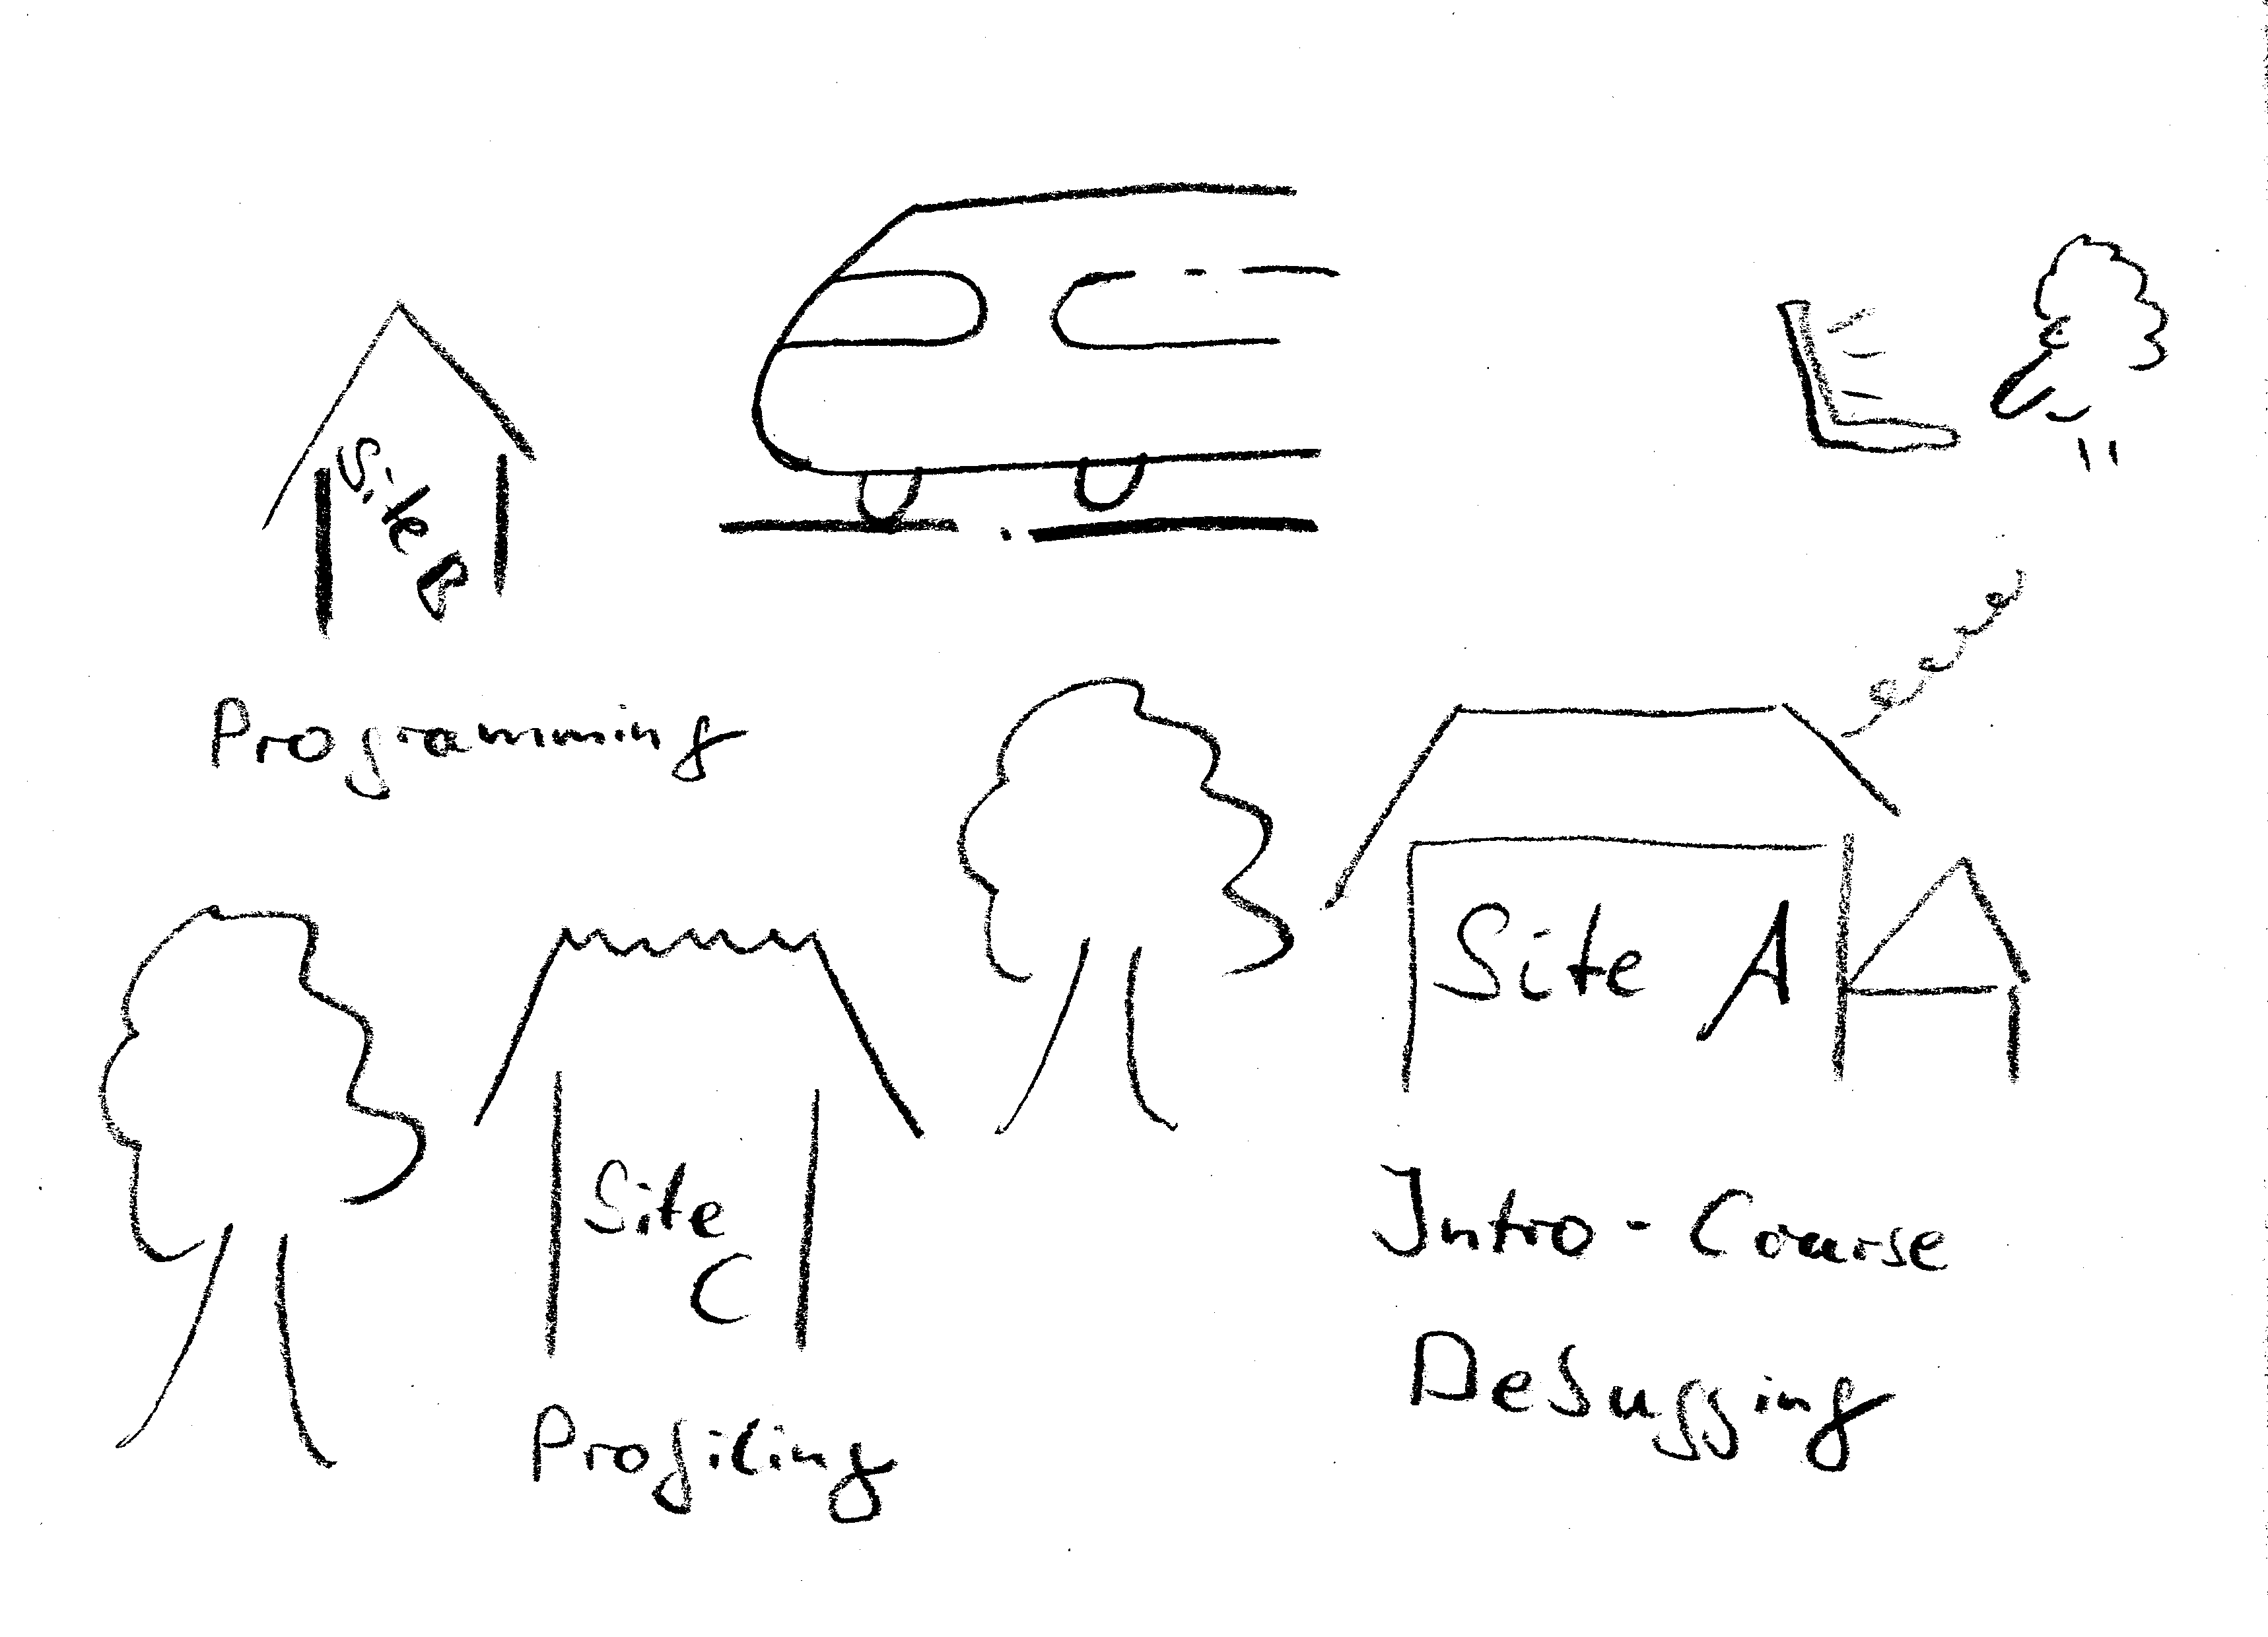
\includegraphics[width=0.8\textwidth]{images/poweruser}
    \end{column}
    \begin{column}{.4\textwidth}
      \pause
      Only power users 
      \begin{itemize}[<+->]
        \item \ldots will select \emph{their} topics \ldots
        \item \ldots will care to travel for computing topics \ldots
        \item \ldots will rarely need intro courses \ldots
      \end{itemize}
    \end{column}
  \end{columns}
\end{frame}

%%%%%%%%%%%%%%%%%%%%%%%%%%%%%%%%%%%%%%%%%%%%%%%%%%%%%%%%%%%%%%%%%%%%%%%%%%%%%%%%
\begin{frame}
  \frametitle{HPCCF a Plus for Power Users}
  \begin{columns}
    \begin{column}{.5\textwidth}
      Advanced Users already use HPC ressources, incl. training. They are aware of
      \begin{itemize}
       \item their local courses
       \item PRACE and other (in-)ternational training resources
      \end{itemize}
    \end{column}
    \begin{column}{.5\textwidth}
      \pause
      Still, they too, will have been newbies at some point \emph{and}
      \begin{itemize}[<+->]
        \item transparency will help them select appropriate courses, too.
        \item ``'Complement my portfolio!''
      \end{itemize}
    \end{column}
  \end{columns}
\end{frame}

\subsection{Certification Process}

\begin{frame}
  \frametitle{Strategy}
  When conceiving a Certification Strategy the different views are in our mind.
  
\end{frame}

\begin{frame}
 \frametitle{Selecting Questions}
 \begin{columns}
    \begin{column}{.5\textwidth}
       \centering
      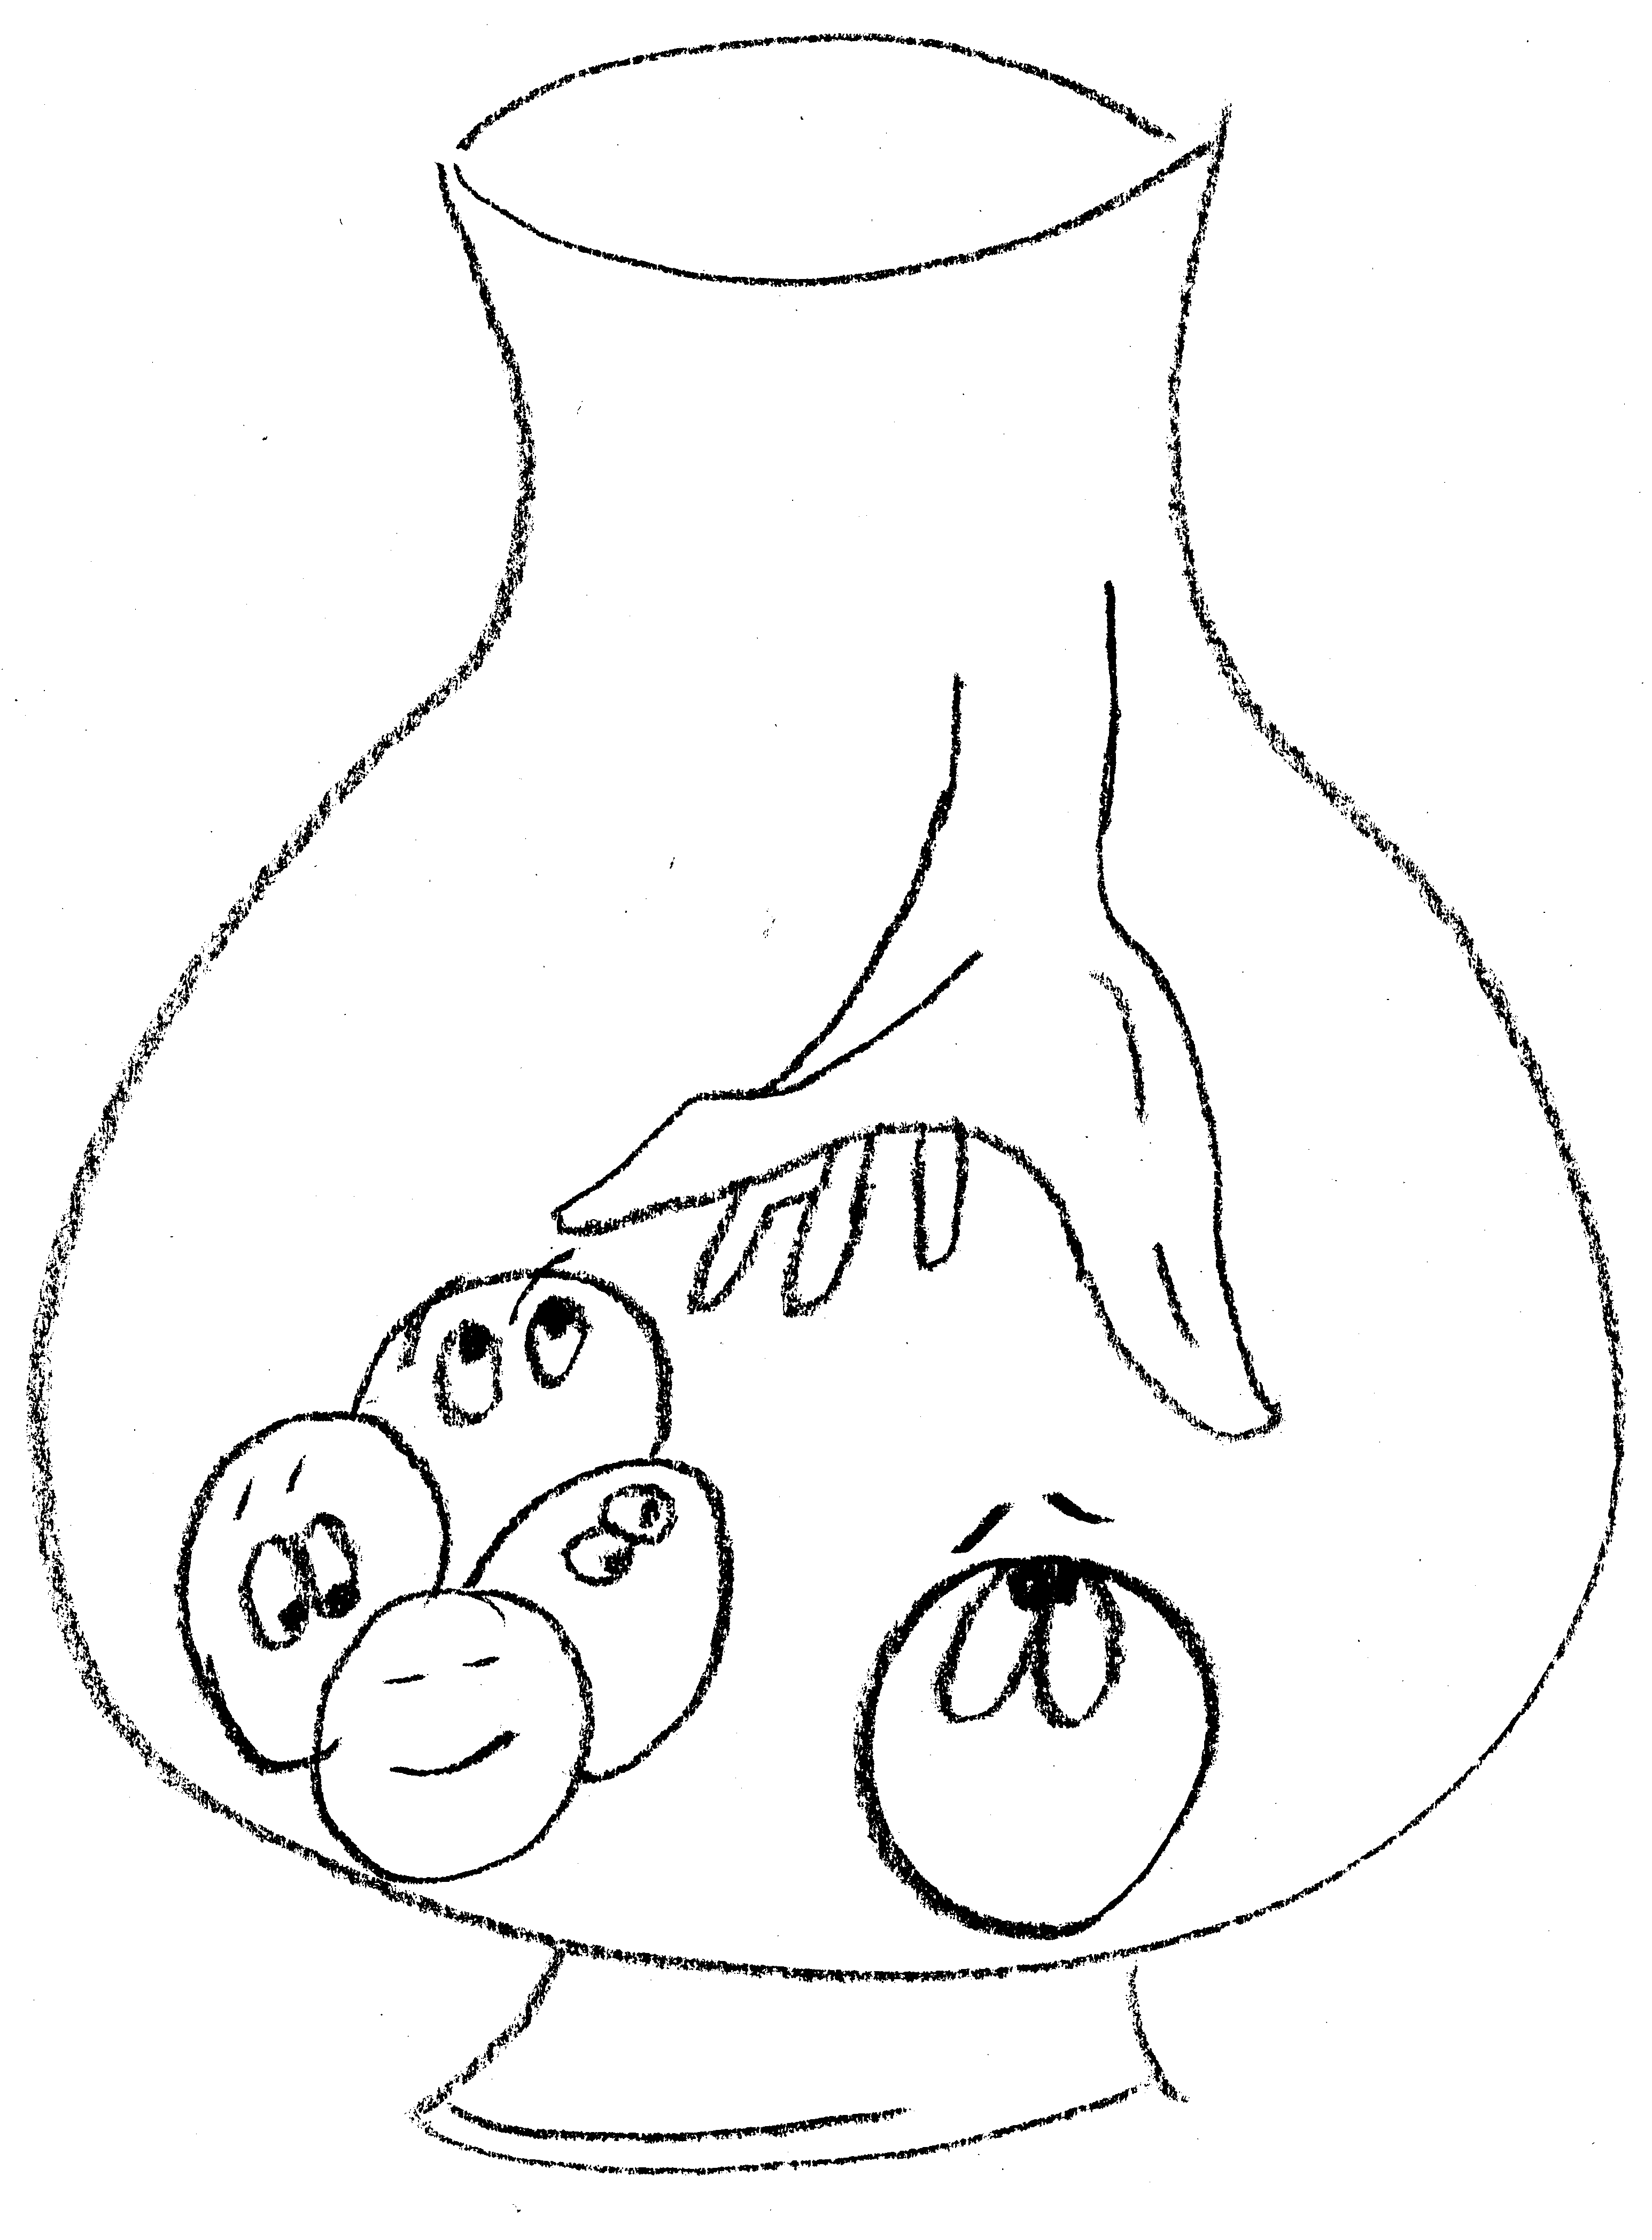
\includegraphics[width=0.6\textwidth]{images/urn}
    \end{column}
    \begin{column}{.5\textwidth}
      Questions are randomly choosen from a pool:
      \begin{itemize}
        \item the pool may itself be a pool of sub-branches of the skill tree
        \item each question will have a pool of right and wrong answers in case of multiple choice questions
      \end{itemize}
      $\curvearrowright$ All examininations will be based on different sets of questions.
    \end{column}
  \end{columns}
\end{frame}

\begin{frame}
  \frametitle{On Cheating}
  \begin{columns}
   \begin{column}{.5\textwidth}
     \begin{enumerate}
      \item By confronting with random questions no perfect preperation can be accomplished.
      \item There is a time-limit per question.
      \item A registration prior to a test session is required.
     \end{enumerate}
    No online system without ID checks and other measures is safe against cheating! Yet, our measures will raise awareness.
   \end{column}
   \begin{column}{.5\textwidth}
       \centering
      
\includegraphics[width=0.6\textwidth]{images/cheating}
    \end{column}
  \end{columns}
\end{frame}

\begin{frame}
 \frametitle{Boosting Acceptance}
 \begin{columns}
   \begin{column}{.5\textwidth}
     Want to hire a scientist? \newline
     We intend to provide a (sub)set of question for prospective employers. This way they will have an idea of the background, if a solicitant waves a HPCCF-certificate.
   \end{column}
   \begin{column}{.5\textwidth}
       \centering
      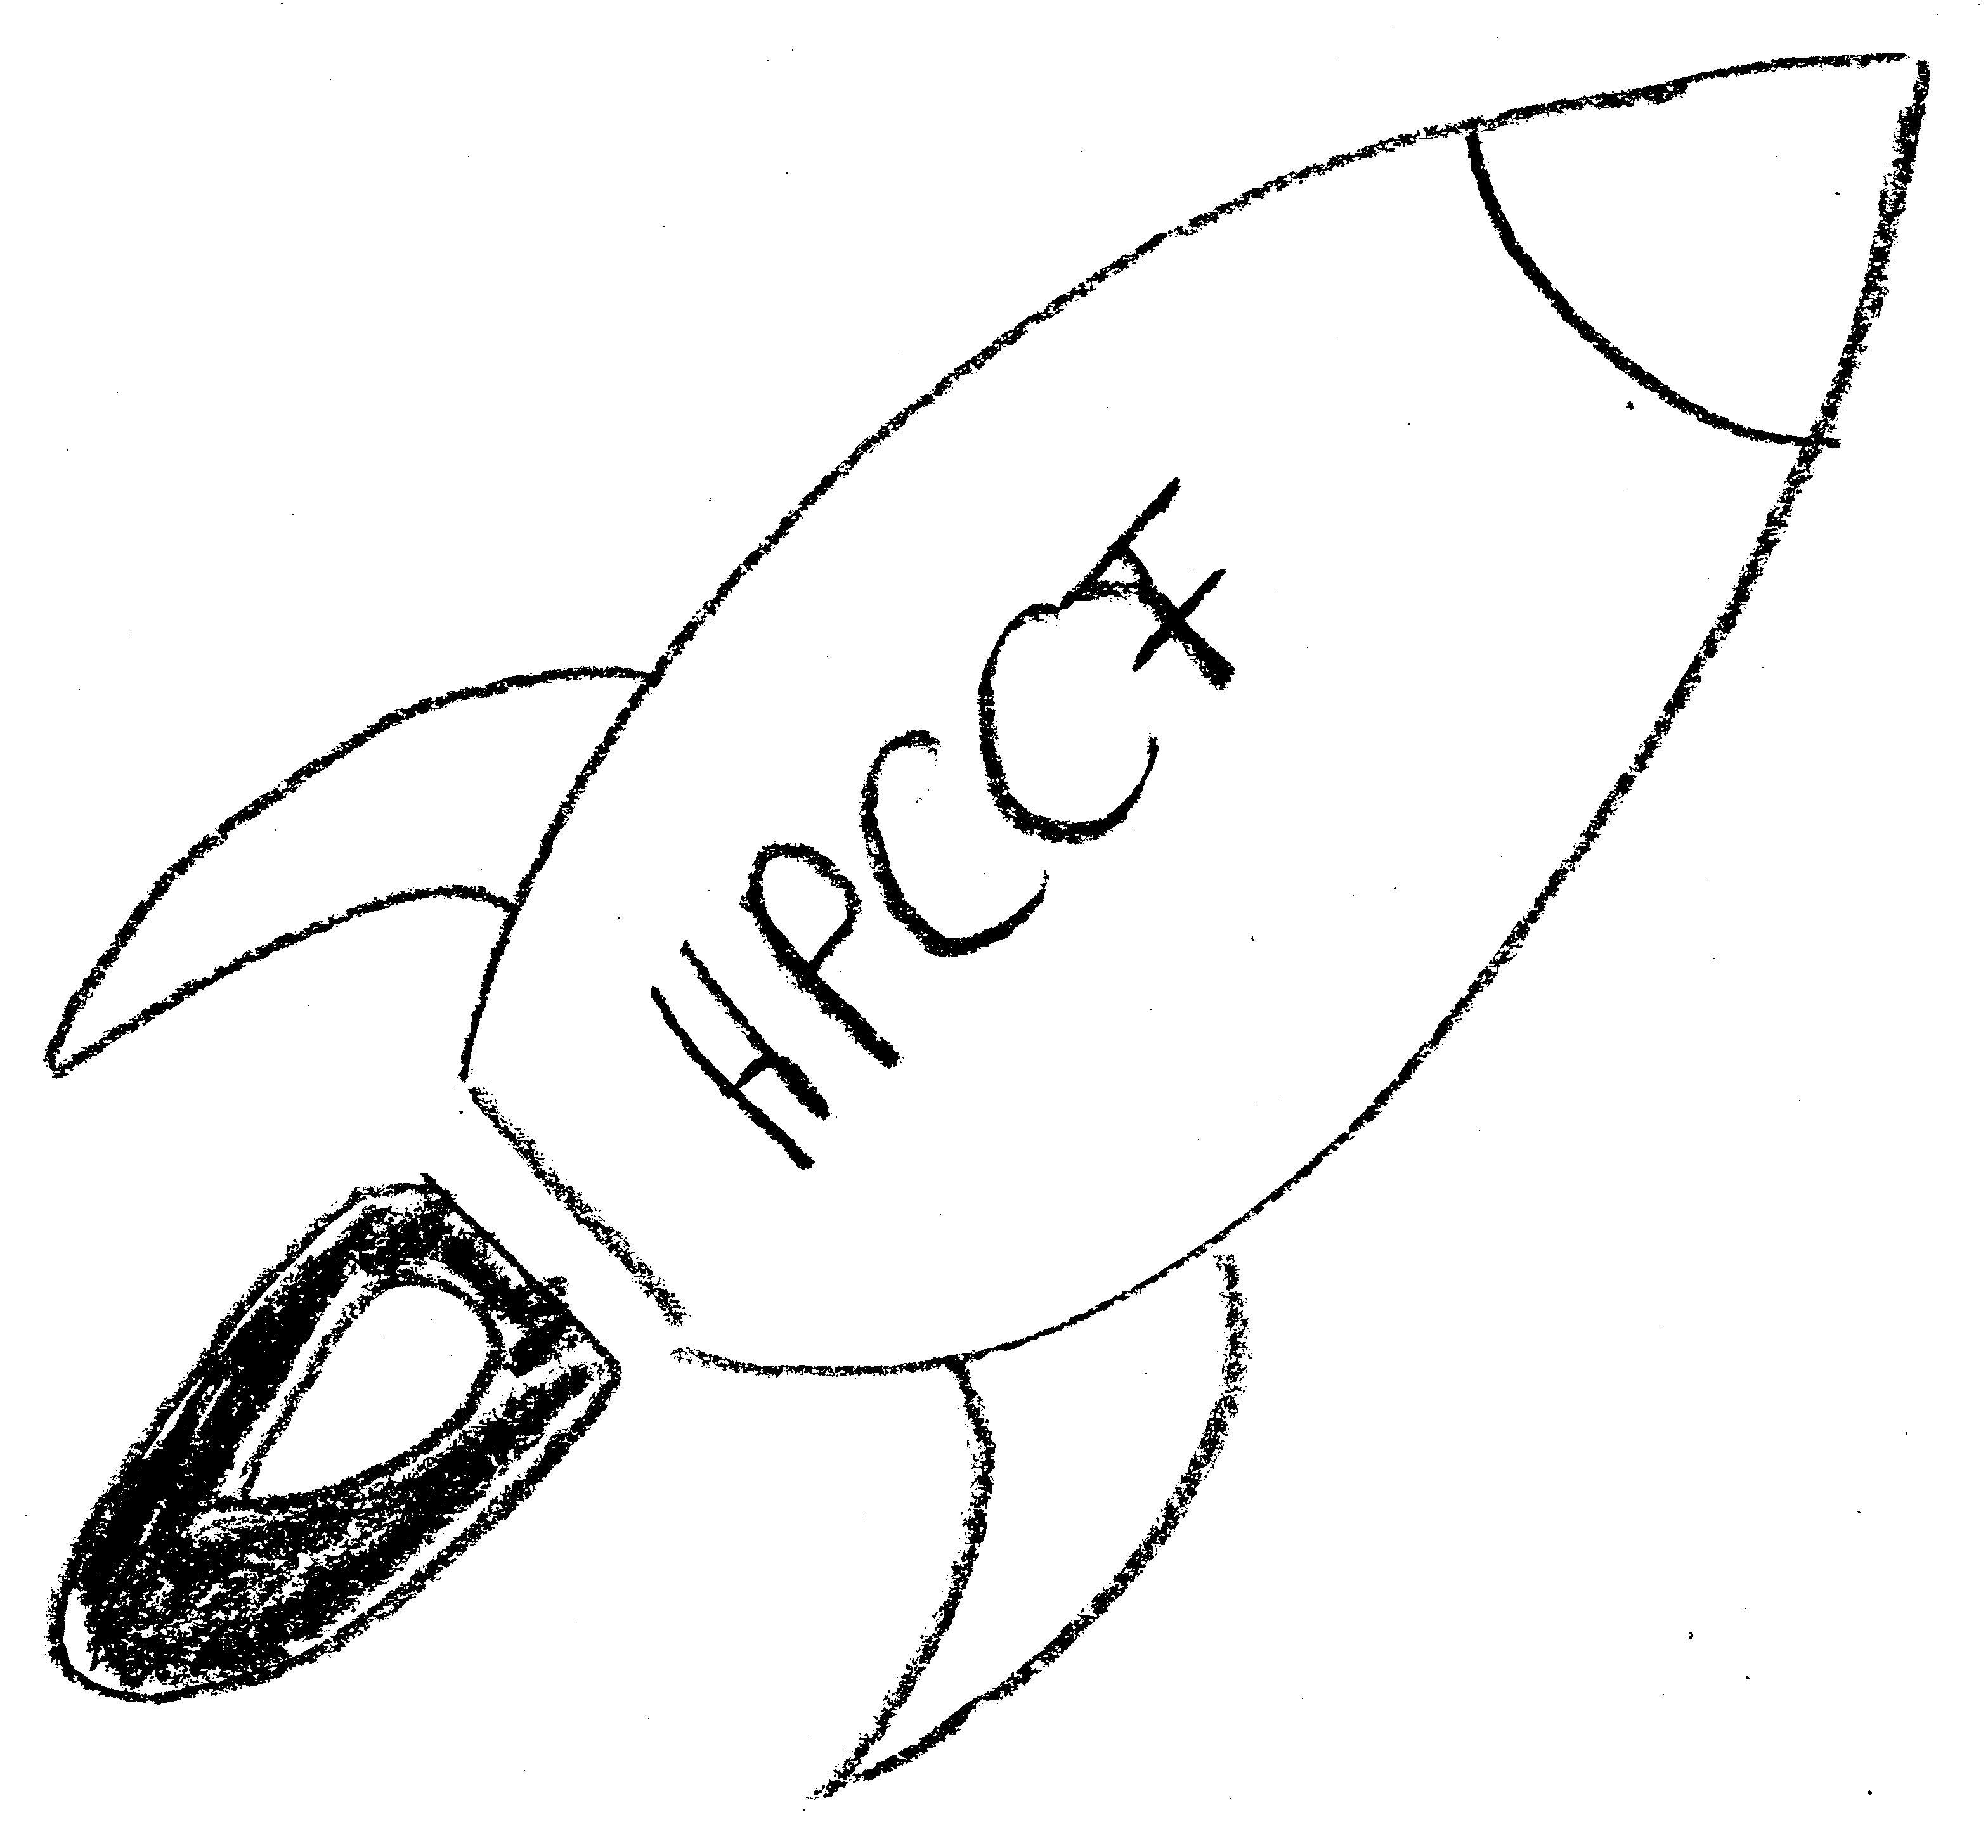
\includegraphics[width=0.6\textwidth]{images/hpccf_boost}
    \end{column}
  \end{columns}
\end{frame}




